% =====================================================================
% 3  METHODS   (draft v1, 2026-11-05; house target 1000--1500 prose words)
% Models and data | design and conditions | measures | procedure |
% data analysis | ethics and preregistration.
% Secondary detail (revision provenance, post-norm derivation, full method
% specifications, search-space table, planned-condition list, seeding and
% prompt-split minutiae, held-out sampling, judge and degeneracy
% implementation, export/release, compute/software, deviations) was moved to
% sections/08b_setup_details.tex (Appendix "Experimental Details",
% label app:setup-details); labels moved with their content.
% Revision 2026-11-05 (review fixes): nominal 100-trial budget with pointer to
% deviations restored; "primary and secondary" restored; dev/KL prompt split
% aligned with 08b; capability subsets vs complete sets corrected; "Proportions"
% restored; planned gamma-corrected control restored; appendix targets now cited
% as "Appendix~\ref". To stay within 1500 words, three details now appear only
% in Appendix app:setup-opt (08b): the list of seeded generators (Python, NumPy,
% PyTorch, Optuna; moved there), the response prefix that closes the reasoning
% block for Qwen3.8-27B/Qwen3.5-4B ("Objective details"), and Heretic's headless
% default selection ignoring KL ("Selection").
% Every factual paragraph/table carries a "% src:" comment; paths are
% relative to the paper-33 root (../heretic = /data/heretic_2/heretic).
% 2026-11-05 (reference integration): cited dodge2019show (budget), zhang2019rmsnorm,
% kim2025periln, gemmateam2024gemma2, walsh2025olmo2, olmo2025olmo3 (post-norm;
% Olmo 3 SWA in tab:models note b), yang2025gated and marshall2024refusal (hybrid
% layers; degeneracy), carleo2026willing (size confound), sainz2023nlp
% (benchmark exposure), huang2024catastrophic (decoding), xie2025sorrybench and
% eiras2025know (WildGuard vs HarmBench classifier: kappa 60.6 vs 52.5; storytelling
% FNR 0.02->0.12 vs 0.12->0.36), evseev2026wrdo (same three judges), brown2001interval,
% miller2024adding, bates2015lme4 (notation only; analysis software still todo),
% baayen2008mixed, cohen1960coefficient, fleiss1971measuring (panel kappa; confirm
% it is computed), feinstein1990high, cawley2010overfitting, cui2025orbench
% (Spearman 0.89 over-refusal vs toxic rejection).
% =====================================================================
\section{Methods}
\label{sec:setup}

The study crosses model generation with refusal-removal method under one
selection rule, one evaluation harness independent of the optimisation
objective and the same nominal budget of 100 trials (exceptions in
Appendix~\ref{sec:setup-deviations}), since method comparisons depend on the
search budget \cite{dodge2019show}; further detail is in
Appendix~\ref{app:setup-details}. Figure~\ref{fig:workflow} summarises the
workflow.
% src: notes/EXECUTION_PLAN_v2.md (Design: "Small pair (4090, free)"; Evaluation protocol); scripts/select_trial.py; scripts/eval_one.sh; configs/core_*.toml (n_trials); scripts/select_trial.py --no-write (qwen3.8-27b__mpoa__core-s1-resume1 99/100)
% 2026-11-06: workflow figure (paper/figures/fig1_workflow.pdf) inserted here when the Results floats were added.

\begin{figure*}[tp]
\centering
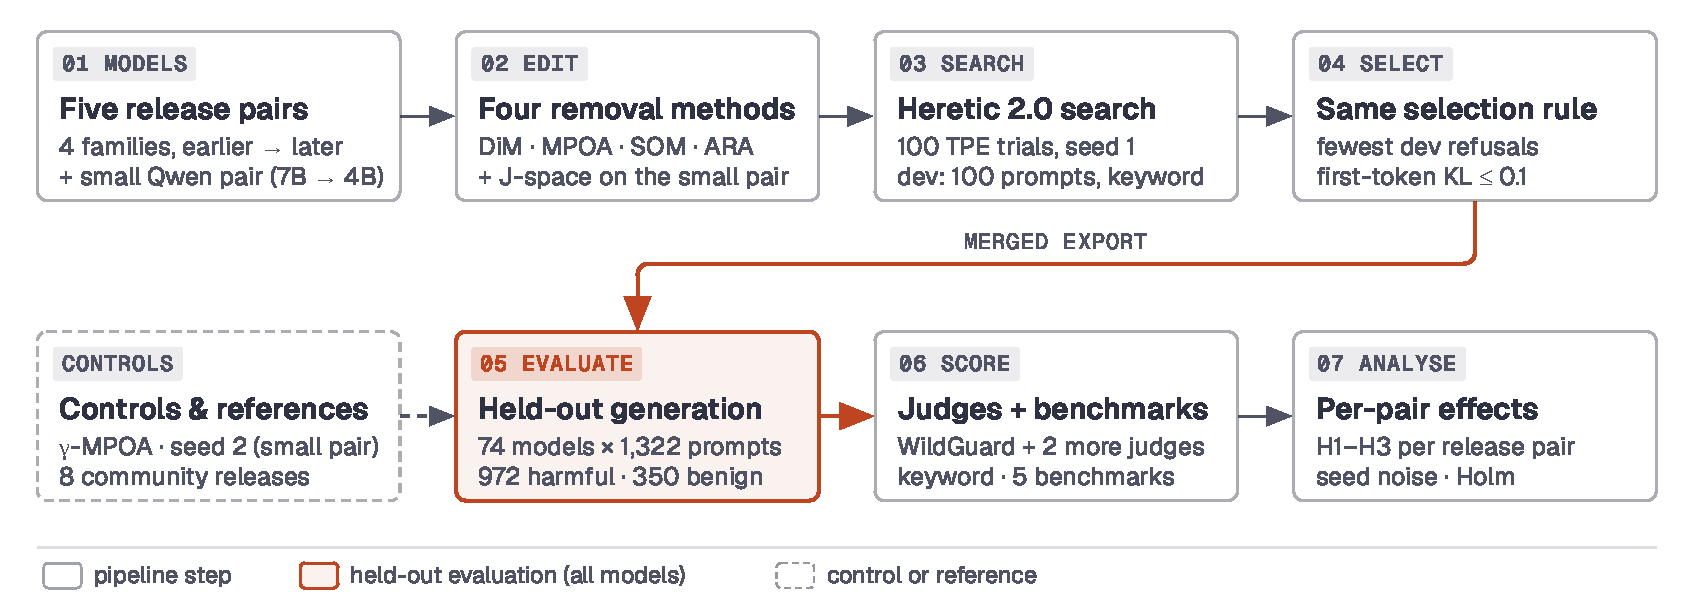
\includegraphics[width=\textwidth]{figures/fig1_workflow.pdf}
\caption{\textbf{Study workflow.} Five earlier-to-later pairs of instruction-tuned models are edited with four refusal-removal methods in Heretic 2.0 (five on the small pair, which adds J-space), each in a 100-trial Optuna TPE study that minimises dev keyword refusals and first-token KL divergence; the trial with the fewest dev refusals at KL $\le$ 0.1 is exported as standalone weights. The originals, the selected models and eight public community abliterations are evaluated on held-out data (judged refusal on 1,322 prompts, of which the 44 that exactly (36) or approximately (8) match a prompt of the search dataset are flagged; teacher-forced divergence on the 350 benign prompts; five capability benchmarks), and the statistics test H1--H3 and compare dev-set with held-out refusal. Dashed boxes mark additional conditions, coloured squares identify methods, and grey notes give the GPUs used for search and evaluation.}
\label{fig:workflow}
\end{figure*}
% caption: paper/figures/captions.md (fig1_workflow)

% ---------------------------------------------------------------------
\subsection{Models and Data}
\label{sec:setup-models}

The main study uses one dense instruction-tuned model per family per
generation, of similar scale, each run unquantised in bf16 on a single GPU
(Table~\ref{tab:models}). The families are Qwen, Gemma, OLMo and Mistral; OLMo
was included because its training data are openly released. Paired models also
differ in size and partly in architecture, and the later model of each pair
was released 9 to 23 months after the earlier one (release months and
checkpoint sizes in Table~\ref{tab:models}).
% src (2026-11-05 todo pass): release months and gaps (9-23 months: OLMo 2025-03 -> 2025-12 and Mistral 2024-09 -> 2025-06 = 9; Qwen 2024-09 -> 2026-08 = 23) from https://huggingface.co/api/models/<repo> (createdAt) and https://huggingface.co/api/models/google/gemma-4-31B-it/commits/main (see tab:models note c)
% src: runs/mc-h200-1/queue.txt; runs/mc-h200-1/queue_b.txt; runs/local-4090/queue.txt; runs/mc-h200-1/models_olmo.txt; runs/mc-h200-1/models_mistral.txt; runs/mc-rtx-1/models_rtx.txt; PLAN.md (Tier B note on OLMo); runs/mc-h200-1/logs/download.log (snapshot paths); runs/mc-rtx-1/results/bench/*__base/summary.json and results/bench-4090/*__base/summary.json (model_info.hf_commit, weights_bytes); runs/mc-h200-1/runs/*/meta.txt (no --model-commit except unsloth mirror)

\begin{table*}[t]
\centering\small
\caption{Models. \emph{Released}: year and month in which the Hugging Face
repository was created (a repository can be created before its public
release; note c). \emph{Revision}: first eight hexadecimal digits of the
Hugging Face commit used. \emph{Size}: bf16 checkpoint size hashed by the
evaluation harness, in GB (image-text checkpoints include their vision
encoder); nominal scale from the repository name in parentheses.
\emph{Layers}: transformer blocks reported by Heretic. Short model names
follow the vendors' spelling (OLMo-2-32B, Olmo-3.1-32B; Mistral-Small-2409 for
\texttt{Mistral-Small-Instruct-2409}); the pairs are labelled Qwen, Gemma, OLMo,
Mistral Small and small pair.}
\label{tab:models}
% layout (2026-11-05 todo pass): narrower column gaps, a wrapped Notes column and scaling to the text width,
% because the table was wider than the text block (overfull by 161 pt before the Released column was added)
\setlength{\tabcolsep}{4pt}
\resizebox{\textwidth}{!}{%
\begin{tabular}{@{}llllllr>{\raggedright\arraybackslash}p{3.1cm}@{}}
\toprule
Family & Gen. & Released & Repository & Revision & Size (GB) & Layers & Notes \\
\midrule
\multicolumn{8}{l}{\emph{Main study}} \\
Qwen    & earlier & 2024-09 & \texttt{Qwen/Qwen2.5-32B-Instruct}                       & \texttt{5ede1c97} & 65.5 (32B) & 64 & -- \\
Qwen    & later   & 2026-08 & \texttt{Qwen/Qwen3.8-27B}                                & \texttt{1d4bf0f2} & 55.6 (27B) & 64 & hybrid linear/full attention; image-text \\
Gemma   & earlier & 2024-06 & \texttt{google/gemma-2-27b-it}                           & \texttt{aaf20e6b} & 54.5 (27B) & 46 & post-norm \cite{gemmateam2024gemma2}; no system role \\
Gemma   & later   & 2026-04$^{c}$ & \texttt{google/gemma-4-31B-it}                     & \texttt{842da379} & 62.6 (31B) & 60 & post-norm; image-text \\
OLMo    & earlier & 2025-03 & \texttt{allenai/OLMo-2-0325-32B-Instruct}                & \texttt{b9602434} & 64.5 (32B) & 64 & post-norm \cite{walsh2025olmo2} \\
OLMo    & later   & 2025-12 & \texttt{allenai/Olmo-3.1-32B-Instruct}                   & \texttt{ac0587e4} & 64.5 (32B) & 64 & post-norm; sliding-window attention$^{b}$ \\
Mistral & earlier & 2024-09 & \texttt{mistralai/Mistral-Small-Instruct-2409}           & \texttt{4600506f} & 44.5$^{d}$ (22B) & 56 & -- \\
Mistral & later   & 2025-06 & \texttt{mistralai/Mistral-Small-3.2-24B-Instruct-2506}$^{a}$ & \texttt{3ed8d341}$^{a}$ & 48.1 (24B) & 40 & image-text \\
\midrule
\multicolumn{8}{l}{\emph{Small pair}} \\
Qwen    & earlier & 2024-09 & \texttt{Qwen/Qwen2.5-7B-Instruct}                        & \texttt{a09a3545} & 15.2 (7B) & 28 & -- \\
Qwen    & later   & 2026-02 & \texttt{Qwen/Qwen3.5-4B}                                 & \texttt{851bf6e8} & 9.3 (4B)  & 32 & hybrid linear/full attention; image-text \\
\bottomrule
\end{tabular}}
% src (2026-11-05 todo pass): Released = createdAt month from https://huggingface.co/api/models/<repo> for each repository in the table (official mistralai repo for Mistral-Small-3.2: 2025-06-19); Gemma-4 2026-04 from https://huggingface.co/api/models/google/gemma-4-31B-it/commits/main (createdAt 2026-03-11; oldest public commit 2026-04-02 "Preparing for release!", community PRs #56/#59 on 2026-04-10)
% src (2026-11-05 todo pass): sizes from model_info.weights_bytes in runs/mc-h200-1/results/bench/{olmo-2-32b,olmo-3.1-32b,mistral-small-3.2}__base/summary.json (64478373025, 64476864279, 48059591600 bytes); Mistral-2409 44.5 = sum of model-0000{1..9}-of-00009.safetensors (44494624536 bytes) in https://huggingface.co/api/models/mistralai/Mistral-Small-Instruct-2409/tree/4600506f6b13c7ef89e61a54263f4c9bf483de30, harness total 88991978665 bytes in runs/mc-h200-1/results/bench/mistral-small-2409__base/summary.json and model_hash.json (includes consolidated.safetensors, 44494620752 bytes); 22B from https://huggingface.co/api/models/mistralai/Mistral-Small-Instruct-2409 (safetensors.total 22247282688)

\smallskip
\footnotesize $^{a}$Loaded from the mirror
\texttt{unsloth/Mistral-Small-3.2-24B-Instruct-2506} at commit
\texttt{3ed8d341}, whose weight shards are byte-identical to the official
repository (Appendix~\ref{sec:setup-deviations}).
$^{b}$On three of every four layers (48 of 64, every fourth layer using full
attention; 4{,}096-token window), as specified by \texttt{layer\_types} and
\texttt{sliding\_window} in the checkpoint's \texttt{config.json} and reported
for Olmo~3 \cite{olmo2025olmo3}.
% src (2026-11-05 todo pass): https://huggingface.co/allenai/Olmo-3.1-32B-Instruct/resolve/ac0587e4a7744a551c059d8cd17ba220bc940dae/config.json (sliding_window 4096; layer_types: 48 sliding_attention, 16 full_attention, pattern 3 sliding + 1 full; num_hidden_layers 64)
$^{c}$The repository was created on 2026-03-11, but its public history begins
with a commit titled ``Preparing for release!'' on 2026-04-02.
$^{d}$Hugging Face-format weight shards only; the repository also holds the
weights in Mistral's native format (\texttt{consolidated.safetensors},
44.5\,GB), so the harness hashed 89.0\,GB in total. The repository name gives
no scale; 22B follows from its 22.2 billion parameters.
\end{table*}
% src: runs/mc-h200-1/logs/download.log; runs/mc-rtx-1/results/bench/{qwen2.5-32b,qwen3.8-27b,gemma-2-27b,gemma-4-31b}__base/summary.json; results/bench-4090/{qwen2.5-7b,qwen3.5-4b}__base/summary.json; runs/mc-h200-1/runs/*__mpoa__core-s1*/output.log; runs/local-4090/*__mpoa__core-s1/output.log; notes/EXECUTION_PLAN_v2.md (finding 6); runs/mc-h200-1/queue.txt (mirror commit); runs/mc-rtx-1/results/bench/qwen3.8-27b__base/bench.log ("Resolved architecture: Qwen3_5ForConditionalGeneration"), runs/mc-rtx-1/results/bench/qwen3.8-27b__base/model_hash.json (preprocessor_config.json), runs/mc-rtx-1/results/bench/qwen3.8-27b__mpoa/model_hash.json (processor_config.json) and bench.log (vision rotary warmup)

Three architectural properties are relevant. Gemma-2, Gemma-4, OLMo-2 and Olmo-3.1
normalise module outputs with an RMSNorm \cite{zhang2019rmsnorm} with
elementwise gain $\boldsymbol{\gamma}$ before they enter the residual stream
(``post-norm'', i.e.\ output normalisation \cite{kim2025periln}, documented for
Gemma~2, OLMo~2 and Olmo~3
\cite{gemmateam2024gemma2,walsh2025olmo2,olmo2025olmo3}), so direction-based edits are
incomplete on four of the eight main-study models; this potential confound is
disclosed rather than corrected in the primary runs, and a
$\boldsymbol{\gamma}$-corrected MPOA control ($\gamma$-MPOA) was run on these
four models as an additional condition (Appendix~\ref{app:setup-methods};
results in \S\ref{sec:res-secondary}). Qwen3.8-27B and Qwen3.5-4B
interleave gated-delta-rule linear-attention layers \cite{yang2025gated} with
full-attention layers, and four checkpoints are image-text
models used with text only (Appendix~\ref{app:setup-models}).
% src: notes/EXECUTION_PLAN_v2.md (finding 6); runs/mc-h200-1/runs/qwen3.8-27b__ara__core-s1/output.log (traceback in transformers/models/qwen3_5/modeling_qwen3_5.py); runs/local-4090/qwen3.5-4b__ara__core-s1/model_kl0.1_t75/config.json (architectures, layer_types); ../heretic/src/heretic/model.py (get_layer_modules: linear_attn.out_proj; _apply_system_role); scripts/eval_one.sh (Gemma-4 limit_mm_per_prompt image 0); scripts/bench/bench.py (render_prompt fallback); runs/mc-rtx-1/results/bench/qwen3.8-27b__base/bench.log (Qwen3_5ForConditionalGeneration); runs/mc-rtx-1/results/bench/qwen3.8-27b__mpoa/model_hash.json (processor_config.json)

The small pair (Qwen2.5-7B-Instruct and Qwen3.5-4B) is the only candidate
pair with instruction-tuned Jacobian lenses, so J-space ablation is restricted
to it; its later model is the smaller one, confounding generation and size
(Appendix~\ref{app:validity}).
% src: notes/EXECUTION_PLAN_v2.md (finding 7; Design: small pair); PLAN.md (Phases: pilot pair); Table tab:models sizes

\paragraph{Prompt data.} Refusal directions, SOM fitting and ARA module
capture use the first 400 training prompts of
\texttt{mlabonne/harmful\_behaviors} and \texttt{mlabonne/harmless\_alpaca}
\cite{zou2023universal,taori2023alpaca}. The first 100 test prompts of
\texttt{harmful\_behaviors} form the development (dev) set for search and
selection, and those of \texttt{harmless\_alpaca} serve the KL objective.
All primary and secondary refusal, capability and teacher-forced outcomes come
from held-out sets. The held-out refusal set, frozen before any held-out response was generated,
contains 1{,}322 prompts, 972 harmful and 350 benign
(Table~\ref{tab:refusal-sets}), from JailbreakBench, XSTest, StrongREJECT,
HarmBench and a code-as-weapon bank
\cite{chao2024jailbreakbench,rottger2024xstest,souly2024strongreject,mazeika2024harmbench,young2026code}
(sampling in Appendix~\ref{app:setup-eval}). The 44 harmful
items that match a \texttt{harmful\_behaviors} prompt are flagged, and results
are reported with and without them.
% src: ../heretic/src/heretic/modifiers/{abliteration,ara,som}.py (good_prompts/bad_prompts train[:400]); ../heretic/src/heretic/scorers/keyword_rate.py (test[:100]); ../heretic/src/heretic/scorers/kl_divergence.py (test[:100]); notes/EXECUTION_PLAN_v2.md (finding 2; Selection: "full Pareto fronts reported"; Distribution shift: "first-token KL (dev)"; Held-out refusal); scripts/bench/refusal_sets.json (meta; Counter of set/kind/source/advbench_overlap); scripts/build_refusal_sets.py; notes/overnight_log.md (22:45, 22:50)

\begin{table}[t]
\centering\small
\caption{Held-out refusal set (\texttt{refusal\_sets.json}, v2). ``Overlap'':
items matching a \texttt{mlabonne/harmful\_behaviors} prompt exactly / fuzzily.}
\label{tab:refusal-sets}
\begin{tabular}{llrr}
\toprule
Subset & Kind & $n$ & Overlap \\
\midrule
JailbreakBench harmful & harmful & 100 & 11 / 6 \\
JailbreakBench benign  & benign  & 100 & -- \\
XSTest unsafe          & harmful & 200 & 0 / 0 \\
XSTest safe            & benign  & 250 & -- \\
StrongREJECT           & harmful & 313 & 25 / 1 \\
HarmBench (standard)   & harmful & 159 & 0 / 1 \\
Code-as-weapon         & harmful & 200 & 0 / 0 \\
\midrule
Total                  &         & 1{,}322 & 36 / 8 \\
\bottomrule
\end{tabular}
\end{table}
% src: scripts/bench/refusal_sets.json (Counter over set, kind, advbench_overlap)

% ---------------------------------------------------------------------
\subsection{Study Design and Conditions}
\label{sec:setup-methods}

The independent variables are model generation (earlier or later release
within a family) and refusal-removal method; for H2, ARA forms the optimisation-based class and the
remaining methods the direction-based class. All methods run inside
Heretic~2.0 \cite{heretic2025} and differ in the weight edit and its search
space (Table~\ref{tab:search}, Appendix~\ref{app:setup-methods}). Each edit targets
the attention output projection and MLP down-projection of each layer and is
held in a LoRA adapter \cite{hu2022lora} during optimisation. The methods of
Appendix~\ref{sec:methods} are instantiated as follows (full specification
and additional conditions in Appendix~\ref{app:setup-methods}). Three presets
of the external OBLITERATUS toolkit \cite{obliteratus2026} on
Qwen2.5-7B-Instruct are evaluated with this study's harness in the companion
paper \cite{young2026paper30} and are not part of this study.
% src (2026-11-06, author decision: OBLITERATUS reported in paper 30 only): results/bench-4090/qwen2.5-7b__obliteratus-{basic,advanced,spectral_cascade}/push_manifest.json; ../paper30/v3_2611/analysis/RESULTS.md
% src: ../heretic/src/heretic/model.py (apply_lora; _zero_lora_weights; get_layer_modules); ../heretic/src/heretic/modifiers/{abliteration,som,ara}.py (suggest_parameters); notes/EXECUTION_PLAN_v2.md (Statistics: method_class; Design)

\paragraph{DiM.} The difference-in-means refusal direction
\cite{arditi2024refusal} is removed by a rank-1 edit that leaves the embedding
matrix unchanged; unlike the original procedure
(Appendix~\ref{sec:m-dim}), direction,
strength and layer profile are tuned by the same search as MPOA
(``Heretic-tuned DiM'').
% src: configs/core_dim.toml; ../heretic/src/heretic/modifiers/abliteration.py (init, suggest_parameters, modify_model; embedding comment); notes/EXECUTION_PLAN_v2.md (Design: Heretic-tuned DiM)

\paragraph{MPOA.} Heretic's defaults: the direction is projected orthogonal to
the harmless mean \cite{lai2024projected}, and the edit is computed on
row-normalised weights whose row norms are then restored \cite{lai2025mpoa}
(rank-3 adapter).
% src: configs/core_mpoa.toml (defaults); ../heretic/src/heretic/modifiers/abliteration.py (orthogonalize_direction=True, row_normalization=FULL, full_normalization_lora_rank=3)

\paragraph{SOM.} A port of the proof of concept in Heretic PR~\#196
\cite{piras2025som} (``Heretic-tuned SOM''): the $k=4$ most-winning neurons of a
per-layer self-organising map of harmful residuals yield orthonormalised
directions, which are ablated with a searched geometric decay (rank-6 adapter).
% src: configs/core_som.toml; ../heretic/src/heretic/modifiers/som.py (Settings, fit_som, count_wins, select_top_k_neurons, orthonormalize, suggest_parameters, compute_lora); notes/overnight_log.md (02:42)

\paragraph{ARA.} Heretic's default modifier \cite{weidmann2026ara}: a rank-50
adapter per targeted module is fitted by L-BFGS to the objective of
Appendix~\ref{sec:m-ara}; row-magnitude preservation enters only the objective, and
the exported adapter is not renormalised.
% src: configs/core_ara.toml (defaults); ../heretic/src/heretic/modifiers/ara.py (Settings, ara_loss, modify_model); notes/EXECUTION_PLAN_v2.md (finding 10)

\paragraph{J-space (small pair only).} Directions computed by the
\texttt{jspace-refusal} code from Jacobian lenses and refusal-token
unembeddings
\cite{sekinal2026jspace,neuronpedia2026jacobian,gurnee2026verbalizable} are
baked into the weights with the DiM/MPOA edit and search space (rank-3 adapter)
rather than applied as the original forward hook.
% src: scripts/jspace_directions.py; directions/{qwen3.5-4b,qwen2.5-7b}__jspace.pt (meta); configs/core_jspace.toml; ../heretic/src/heretic/modifiers/precomputed.py; env/env_4090-omarchy.txt (jspace-refusal 30a1b9c)

% ---------------------------------------------------------------------
\subsection{Measures}
\label{sec:setup-eval}

\paragraph{Generation.} One response per held-out prompt is generated for the
original and every modified model with vLLM \cite{kwon2023efficient}:
greedy, at most 512 new tokens, the model's own chat template, system prompt
``You are a helpful assistant.'' and reasoning disabled. Decoding is
identical for all models because refusal is highly sensitive to decoding
settings \cite{huang2024catastrophic}.
% src: scripts/bench/refusal_sets.json (meta: system_prompt, max_tokens 512, greedy); scripts/bench/bench.py (render_prompt, generate_refusal_set)

\paragraph{Refusal and outcome classes.} The primary outcome is the
WildGuard \cite{han2024wildguard} refusal label of each harmful held-out
response; WildGuard agreed more closely with human labels than the HarmBench
classifier and was less affected by stylistic rewriting
\cite{xie2025sorrybench,eiras2025know}. All judges score the same stored responses: WildGuard (refusal and
harmful response), the HarmBench classifier (harmful compliance),
Qwen3Guard-Gen-8B \cite{zhao2025qwen3guard} (second LLM judge), two
encoder-based refusal classifiers, and Heretic's 33 keyword markers on the full
response and its first 256 tokens; WildGuard, Qwen3Guard and the HarmBench
classifier were also used by a recent refusal-direction study
\cite{evseev2026wrdo}. A degeneracy heuristic flags empty, repetitive or
largely non-printable responses, which ablation can produce
\cite{marshall2024refusal}. Each response is assigned one outcome class in a
fixed order: degenerate if flagged, otherwise refusal if WildGuard labelled it
a refusal, otherwise compliance, split into complete and incomplete compliance
by whether generation stopped at the 512-token limit (finish reason
\texttt{length}). The primary outcome uses the WildGuard label of every
response, degenerate ones included; in the outcome classes degenerate
responses count as not refused (Appendix~\ref{app:setup-eval}).
% src (2026-11-05 todo pass): scripts/analysis/assemble.py (docstring "OUTCOME RULE"; derive(): np.select order degenerate -> unscored -> refusal -> compliance; incomplete = finish_reason == "length"; outcome4 splits compliance only); results/analysis/README.md ("Outcome rule"); scripts/analysis/h1h2.py (wg = ref_wg PRIMARY; wg_class: degenerate = not refused)
% src: scripts/bench/score_refusals.py (docstring, KEYWORDS, keyword(), degenerate(), run_bert, run_vllm, judge calls); scripts/bench/judge_templates/; notes/EXECUTION_PLAN_v2.md (Statistics; Judges: WildGuard primary; finding 3)

\paragraph{Capability and distribution shift.} Five benchmarks run with
lm-evaluation-harness 0.4.13 \cite{gao2024language} on vLLM 0.33.0
(Table~\ref{tab:capability}): fixed, seeded subsets of MMLU-Pro
\cite{wang2024mmlupro} and GSM8K \cite{cobbe2021training} and the complete
IFEval \cite{zhou2023instruction}, HumanEval \cite{chen2021evaluating} and MBPP
\cite{austin2021program} test sets, with greedy decoding, chat templates and
reasoning disabled. Distribution shift is measured by the first-token KL
divergence of the distance objective (\S\ref{sec:setup-opt}) and by a
teacher-forced divergence: the original model's non-empty greedy responses $y$
to the 350 benign held-out prompts are scored by each model, and the divergence
of a modified model is the token-averaged
$\log p_{\mathrm{orig}}(y)-\log p_{\mathrm{mod}}(y)$.
% src: scripts/bench/README.md (Protocol; table: MMLU-Pro 1000 stratified, GSM8K 500 random of 1319, IFEval 541 full, HumanEval 164 full, MBPP 500 test full); scripts/bench/bench.py (BENCHMARKS, SEEDS, build_lm, verify_ids; teacher_forced_logprobs; kind == "benign"); scripts/bench/subsets.json (seed 20261104); runs/mc-rtx-1/results/bench/qwen3.8-27b__mpoa/summary.json (teacher_forced.n_items 350)

\begin{table}[t]
\centering\small
\caption{Capability benchmarks: lm-eval task, items, shots, primary metric and
maximum generated tokens.}
\label{tab:capability}
\begin{tabular}{llrrlr}
\toprule
Benchmark & Task & $n$ & Shots & Metric & Max.\ tok. \\
\midrule
MMLU-Pro  & \texttt{mmlu\_pro\_*}        & 1{,}000 & 5 (CoT) & exact match & 2{,}048 \\
GSM8K     & \texttt{gsm8k}               & 500     & 5 & exact match (flexible) & 512 \\
IFEval    & \texttt{ifeval}              & 541     & 0 & prompt-level strict acc. & 1{,}280 \\
HumanEval & \texttt{humaneval\_instruct} & 164     & 0 & pass@1 & 1{,}024 \\
MBPP      & \texttt{mbpp\_instruct}      & 500     & 3 & pass@1 & 1{,}024 \\
\bottomrule
\end{tabular}
\end{table}
% src: scripts/bench/README.md (Protocol table: GSM8K 500 random of 1319, MMLU-Pro stratified by subject); scripts/bench/bench.py (BENCHMARKS)

% ---------------------------------------------------------------------
\subsection{Procedure}
\label{sec:setup-opt}

\paragraph{Optimisation.} Each model--method combination is one Optuna study
\cite{akiba2019optuna} with a multivariate TPE sampler
\cite{bergstra2011algorithms}: 100 trials, of which the first 30 are random,
with seed~1 (seeded generators, exceptions for two resumed studies and
response-prefix handling in Appendix~\ref{app:setup-opt}). The ten small-pair
studies were repeated with seed~2 to estimate seed sensitivity
(Appendix~\ref{app:setup-methods}). Two objectives are minimised, so each study
yields a Pareto front. The refusal objective is the fraction of 100 greedy
dev-set responses (at most 100 new tokens) containing any of Heretic's 33
refusal markers; the distance objective is the KL divergence of the modified
model's first-token distribution from the original model's, averaged over the
100 harmless prompts.
% src: ../heretic/src/heretic/main.py (TPESampler n_startup_trials, multivariate=True, seed; transformers.set_seed); ../heretic/src/heretic/config.py (n_trials, n_startup_trials, seed, max_response_length=100, system_prompt); configs/core_*.toml; runs/mc-h200-1/queue.txt, queue_b.txt (--seed 1); ../heretic/src/heretic/scorers/keyword_rate.py (REFUSAL_MARKERS); ../heretic/src/heretic/scorers/kl_divergence.py (F.kl_div log_target batchmean); ../heretic/src/heretic/model.py (do_sample=False); runs/mc-h200-1/runs/qwen3.8-27b__*/output.log ("Extended prefix found: '</think>\n'"), runs/local-4090/qwen3.5-4b__*/output.log ("Extended prefix found: '</think>\n\n'")

\paragraph{Selection rule.} One rule is applied to every run: among completed trials
with first-token KL divergence $\le 0.1$, select the one with the fewest dev-set refusals, breaking ties by
lower KL divergence and then lower trial index; if none qualifies, select
nothing and report the lowest-KL trial. For sensitivity analysis the rule is repeated at thresholds 0.05,
0.2 and 0.5, and full Pareto fronts are reported. The cap is the same for
every model, but it need not constrain every run: it is said to bind in a run
when some trial above KL 0.1 had fewer dev refusals than the selected trial.
Binding is recorded for every run, together with the position of the selected
trial's parameters in Heretic's search ranges (Appendix~\ref{app:kl-cap}).
% src: scripts/select_trial.py (docstring, RULE_TEXT, KL_MAX=0.1, REPORT_THRESHOLDS, select()); notes/EXECUTION_PLAN_v2.md (Selection)
% src (review revision, A2): scripts/analysis/review_selection.py docstring (1) ("Cap binding" definition; parameter positions
% src: from the Optuna journals); results/analysis/review_sel_kl_runs.csv, review_sel_kl_params.csv.

\paragraph{Export and release.} Each selected trial is merged into a
standalone checkpoint that differs from the original only in the edited
matrices; the 42 primary models and the four $\gamma$-MPOA controls are
published on Hugging Face, and the ten seed-2 replicates are evaluated but not
released (Appendix~\ref{sec:setup-export}).
% src: scripts/select_trial.py (patch_journal, reexport_commands: --export-strategy MERGE); ../heretic/src/heretic/model.py (get_merged_model: merge_and_unload); scripts/eval_one.sh (publish branch); scripts/publish_local.sh; results/bench-4090/*/publish_check.json ("private": false)

% ---------------------------------------------------------------------
\subsection{Data Analysis}
\label{sec:setup-stats}

All intervals are 95\%. Proportions carry Wilson score intervals
\cite{wilson1927probable,brown2001interval}; paired differences on the same prompts
carry Newcombe's hybrid score intervals \cite{newcombe1998improved} and are
tested with the exact McNemar test \cite{mcnemar1947note}, a paired,
prompt-level comparison as recommended for language-model evaluations
\cite{miller2024adding}. Each modified model is compared in this way with its
original. For H1, the generation effect of a pair and method is the paired
difference in residual refusal between the selected models of the newer and
the older release on the same 972 harmful prompts, tested by exact McNemar.
Pooled over the four main-study families, H1 and H2 are tested with a logistic
generalised estimating equation (GEE) \cite{liang1986longitudinal} with
generation, method class, their interaction and family as fixed effects, an
exchangeable working correlation clustered by prompt and robust standard
errors. The planned mixed-effects logistic regression,
\texttt{refusal $\sim$ generation $\times$ method\_class + (1|prompt) + (1|family)}
in lme4 notation \cite{bates2015lme4,baayen2008mixed}, was fitted by
variational Bayes and is reported as posterior means with $\pm 1.96$~SD
intervals, without $p$ values; its conditional coefficients are larger in
magnitude than the population-averaged GEE coefficients. H1 is tested by the GEE
generation effect within each method class and H2 by the generation $\times$
class interaction, pooled and per pair. H2 is also expressed as a
risk-difference contrast (ARA generation effect minus the mean of the
direction-based methods), and baseline-adjusted generation effects subtract
the originals' own generation difference; both carry item-bootstrap intervals
(4,000 resamples). Pooled baseline-adjusted generation effects come from the
same GEE with the originals added as a reference class, so that the
generation coefficient of each method class is its generation effect minus
that of the originals, in log-odds.

Because each main-study cell was optimised once, these intervals reflect
prompt sampling only, not run-to-run variation of the search. That variation
was estimated post hoc from the ten small-pair cells, each optimised with two
seeds: with $d_i$ the seed-2 minus seed-1 held-out refusal of cell $i$ in
percentage points, the run-to-run standard deviation of one cell is
$\sigma=\sqrt{\sum_{i=1}^{n} d_i^2/(2n)}$ ($n=10$), with a $\chi^2_{10}$
interval, and the difference between two independently optimised cells has
standard deviation $\sigma\sqrt{2}$. A per-pair generation effect is flagged
as exceeding seed noise when its absolute value is larger than
$2\sigma\sqrt{2}$. This flag is a screen that accompanies, not replaces, the
McNemar tests, and it assumes that the seed variability of the 4B and 7B
small-pair models transfers to the 22--32B main-study models. In 3 of the 10
seed pairs (Qwen3.5-4B DiM, SOM and ARA) the seed-2 run also used a generation
batch size of 64 instead of 128, because 128 ran out of memory, so $\sigma$ is
also reported without these pairs.
% src (2026-11-06 reframe): scripts/analysis/seednoise_flags.py -> results/analysis/seednoise_{sigma,flags,summary}.*
% (inputs final_seed_cells.csv, h1h2_generation_effects.csv); h1h2.py gee_with_originals
% ("y ~ C(cls3, Treatment('original')) * gen_new + C(family)", exchangeable, clustered by prompt).
% src (review revision, B1): results/analysis/review_sel_seed_runs.csv (output.log: "Chosen batch size: 64" after CUDA OOM in
% src: qwen3.5-4b__{dim,som,ara}__core-s2; 128 in every other run); review_sel_seed_sigma.csv.

The generational question has the model pair as its unit: four main-study
pairs and one small pair. The prompt-level intervals and tests above
therefore describe prompt sampling within a pair, not variation between runs
or between pairs, and per-pair effects are the primary evidence. For each pair
the generation effect of the direction-based class (the mean of its methods)
and of ARA is given in percentage points (mean of the paired item differences)
and in log-odds (per-pair GEE), raw and baseline-adjusted, with intervals that
add run-to-run variance: each optimised cell contributes $\sigma^2$, so a
single-method effect has $2\sigma^2$, a mean of $m$ methods $2\sigma^2/m$
and the H2 contrast $2\sigma^2+2\sigma^2/m$, with $\sigma$ estimated on each
scale from the seed pairs. Differences between families are tested with Wald
tests of the generation $\times$ family and generation $\times$ class
$\times$ family terms of the GEE (3 df). Pooled effects over the four main
pairs are summarised with a random-effects model: DerSimonian--Laird
between-pair variance \cite{dersimonian1986meta}, a
Hartung--Knapp--Sidik--Jonkman 95\% interval with a $t$ distribution on 3
degrees of freedom \cite{hartung2001refined,inthout2014hartung}, $I^2$
\cite{higgins2002quantifying} and a 95\% prediction interval for a new pair
\cite{higgins2009reevaluation}; with $k=4$ pairs these intervals are wide by
construction. Leave-one-family-out GEE fits complete the pooled analysis. The
baseline-adjusted contrasts were added after H1 had been stated and are
exploratory; because the percentage-point and log-odds scales can disagree in
sign, both are reported.
% src (review revision, A1, C1): scripts/analysis/review_selection.py docstring (2) and "Statistical conventions" (per-pair pp =
% src: mean of paired item differences; log-odds from per-pair GEE; seed variance sigma^2 per optimised cell, 2 sigma^2,
% src: 2 sigma^2 / m, 2 sigma^2 + 2 sigma^2 / m; DL tau^2, HKSJ with t(k-1), prediction interval t(k-2) (Higgins, Thompson &
% src: Spiegelhalter 2009); leave-one-family-out = final.analysis_g); outputs review_sel_pair_{effects,meta,heterogeneity,lofo}.csv,
% src: review_sel_scales.csv.

H3 compares keyword and judge labels on identical responses: the paired
keyword-minus-WildGuard gap of each model (Newcombe interval, exact McNemar),
pooled gaps with prompt-cluster bootstrap intervals (2,000 resamples), and
agreement as Cohen's $\kappa$ for rater pairs \cite{cohen1960coefficient} and
Fleiss' $\kappa$ across judge panels \cite{fleiss1971measuring}, each with a
prompt-bootstrap interval, raw agreement and label marginals, because $\kappa$
is low when labels are as imbalanced as near-0 or near-100\% refusal
\cite{feinstein1990high}. The method-class difference in the gap is tested
with a linear GEE on the per-response paired difference (clustered by prompt,
pair as a fixed effect) and checked with an ordinary least-squares model on
the per-model mean gaps, with the model as unit. Keyword labels are computed
on three windows: the full response (at most 512 tokens), its first 256 tokens
and its first 100 tokens, the window Heretic scores during search. Token ids
were not stored, so the 100-token text is obtained by re-tokenising each
stored response with the evaluated model's tokenizer, a procedure validated
against the stored 256-token prefixes (Appendix~\ref{app:trunc256}).
% src (review revision, C4): scripts/analysis/review_outcomes.py docstring (C4, Tokenisation); heretic config.default.toml @ 8fd4d76
% src: (max_response_length = 100); results/analysis/review_out_checks.csv (re-tokenised 256-token cut reproduces keyword_refusal_256).

Holm's procedure \cite{holm1979simple} controls each family of related tests
at a two-sided $\alpha=0.05$, separately for each refusal measure and prompt
subset (families and sizes in Appendix~\ref{app:setup-stats}).
Variational-Bayes results are not adjusted. Overfitting of selection to the
dev set, expected when a noisy criterion is both optimised and used for
selection \cite{cawley2010overfitting}, is assessed by the Spearman
correlation between dev-set keyword refusal and held-out judged refusal across
selected models, with percentile bootstrap intervals over models. Of the
secondary outcomes (over-refusal on the 350 benign items, which tracks
harmful-prompt refusal across models \cite{cui2025orbench}, capability
differences and teacher-forced divergence), changes in over-refusal from the
original are tested by exact McNemar, Holm-adjusted over all modified models;
the others are descriptive apart from the tests listed above. As
sensitivity analyses, H1 and H2 are repeated on the four public item sets
(772 prompts) and on the code-as-weapon bank (200) separately, and with
harmful compliance as the outcome (HarmBench classifier and WildGuard
harmful-response labels, coded as not harmful so that signs match the refusal
analysis). Dev-set drift of the released exports is compared between exports
rebuilt on the search machine and on another GPU with Fisher's exact test.
These analyses, the pair-level pooling and the KL-cap analysis were added
after the held-out results were known. Analyses used
Python~3.12.15 with pandas~3.1.1, NumPy~2.5.4, SciPy~1.18.1 and
statsmodels~0.15.0 \cite{seabold2010statsmodels}; hardware and other software
versions are listed in Appendix~\ref{sec:setup-compute}.
% src: notes/EXECUTION_PLAN_v2.md (Statistics; Judges: WildGuard primary); paper/sections/02_introduction.tex (H1-H3)
% src (review revision, C2, C3, A3): scripts/analysis/review_outcomes.py docstring (C2: public4 772 items, code_weapon 200; C3:
% src: hbnc / wghnc "not harmful"); scripts/analysis/review_selection.py docstring (5) and review_sel_export_tests.csv (Fisher
% src: exact); review_sel_summary.md / review_out_summary.md generated 2026-11-06T23:44Z / 2026-11-07 00:08Z, after the held-out
% src: results (run_all.sh re-run 06:10:27Z).
% src (2026-11-06 fact-check pass): scripts/analysis/h1h2.py docstring (Newcombe hybrid score CI; exact McNemar;
% planned model = BinomialBayesMixedGLM.fit_vb, mean +/- 1.96 SD, no p; GEE logistic, exchangeable by prompt, robust SE,
% family fixed; Holm families H1 / H2 / ablation, ALPHA = 0.05); results/analysis/h1h2_summary.md (item bootstrap 4000,
% software versions; "R is not installed"); h1h2_tests.csv (n_in_family 23 / 6 / 42); scripts/analysis/h3.py (B = 2000
% prompt-cluster bootstrap; smf.gee Gaussian exchangeable groups=pid + C(pair, Sum); OLS on per-cell mean gaps; Holm
% over 4 GEE terms; per-cell gap Holm across all judged cells); scripts/analysis/final.py (Holm 4 gamma-MPOA vs MPOA;
% 4 per community release; 10 seed cells; 20 per benchmark reference: original, mpoa); scripts/analysis/secondary.py
% (over-refusal McNemar, Holm over all modified cells; Spearman with cell bootstrap)

% ---------------------------------------------------------------------
\subsection{Ethics and Preregistration}
\label{sec:setup-ethics}

\paragraph{Ethics.} No human participants were involved.
% 2026-11-07: todo removed (author: statements final); revise if a human validation sample of the judges is added.
Prompt sets are described by name and count only; responses to harmful prompts
are stored privately for scoring and not released. Licences of released
models and judges are listed in Appendix~\ref{sec:setup-export}.
% src: notes/EXECUTION_PLAN_v2.md (Publishing)

\paragraph{Preregistration.} The study was not preregistered; the hypotheses
were formulated after pilot runs on the small pair (30 trials, 10 random),
which served to verify the pipeline and are not among the analysed runs. The
baseline-adjusted contrast was added after H1 had been stated, and the
pair-level pooling, the KL-cap, item-source and harmful-compliance analyses
and the 100-token keyword window were added after the held-out results were
known; all of these are exploratory.
Deviations from the study plan are listed in
Appendix~\ref{sec:setup-deviations}.
% src: notes/EXECUTION_PLAN_v2.md ("Not preregistered (hypotheses written after pilot data)"); configs/pilot_*.toml; notes/RUNBOOK.md (Pilot first at 30 trials); runs/mc-h200-1/queue.txt (pilot-s1 runs)
